\section{ProblemStatement}

\begin{frame}
	\frametitle{Multi-Object Detection and Tracking}
	\framesubtitle{A brief overview}
	
	\begin{columns}[t]
		\column{0.65\textwidth}
		\centering
		
		\vspace{0.4cm}
		
		\begin{block}{Moving Object Detection}
			real-time extraction of moving objects from sensors
		\end{block}
		
		\vspace{1.3cm}
		
		\begin{block}{Object Tracking \cite{Yilmaz06}}
			continuous observation of the objects over time to form persistent trajectories of the objects
		\end{block}
		
		\column{0.3\textwidth}
		\centering
		
		\begin{tikzpicture}
			\node at (0,0) [draw=black,ultra thick,inner sep=0pt]  {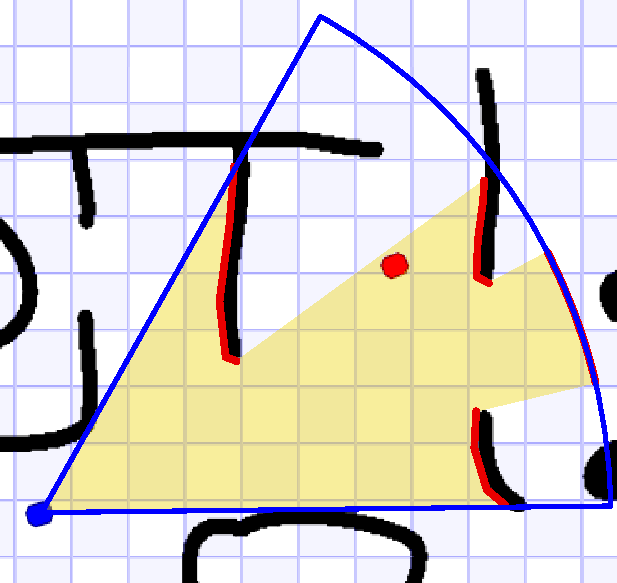
\includegraphics[scale=0.3]{images/Agent}};
		\end{tikzpicture}
		
		\vspace{0.3cm}
		
		\begin{tikzpicture}
			\node at (0,0) [draw=black,ultra thick,inner sep=0pt] {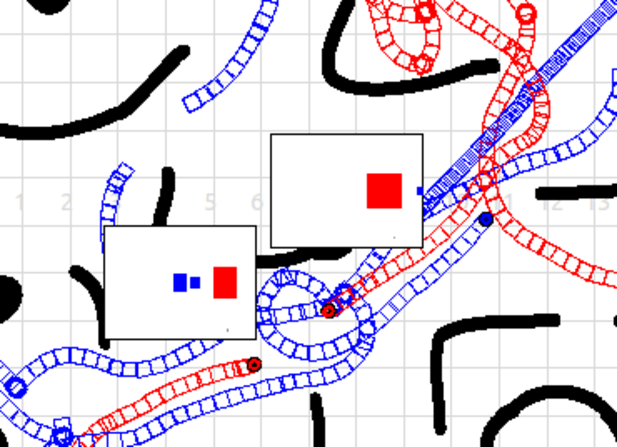
\includegraphics[scale=0.35]{images/Stage}};
		\end{tikzpicture}
	\end{columns}
	
	\vspace{-0.4cm}
	
	\begin{columns}
		\column{1.0\textwidth}
		
		\vspace{0.6cm}
		
		\tiny 5. \emph{Yilmaz et al., ``Object tracking: A survey'' in Journal ACM Computing Surveys (CSUR), 2006}
	\end{columns}
\end{frame}

\begin{frame}
	\frametitle{A distributed lifelong system for the Distributed Multi-Agent Multi-Object Tracking challenge}
	
	\vspace{0.5cm}
	\centering
	
	\begin{tikzpicture}
		\node at (0,0) [draw=white,ultra thick,inner sep=0pt] {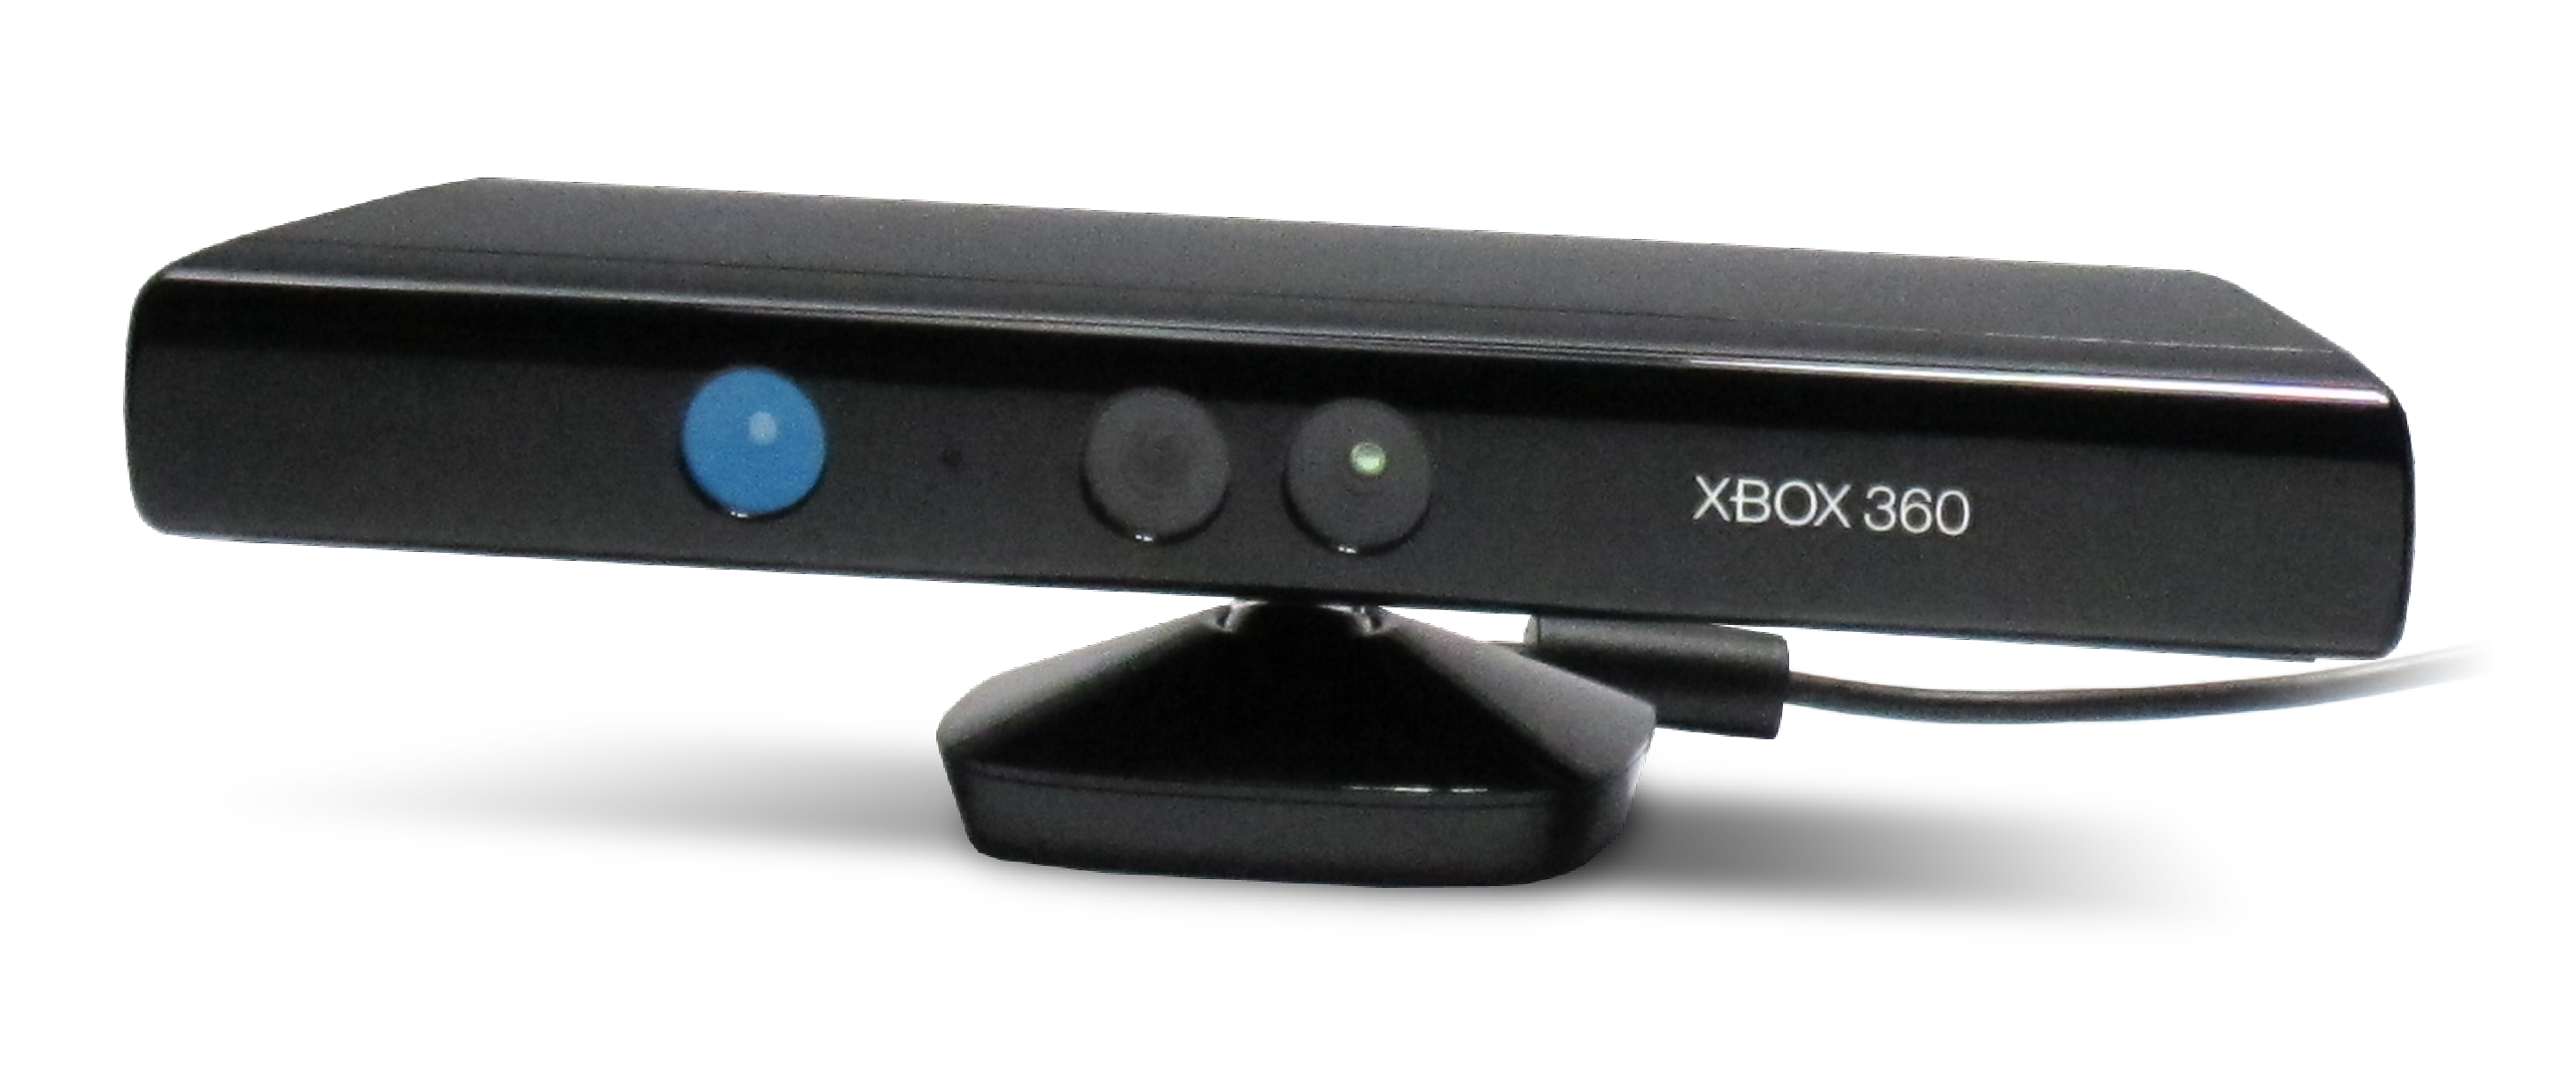
\includegraphics[scale=0.1]{images/Kinect}};
		\node at (3.5,0) [draw=white,ultra thick,inner sep=0pt] {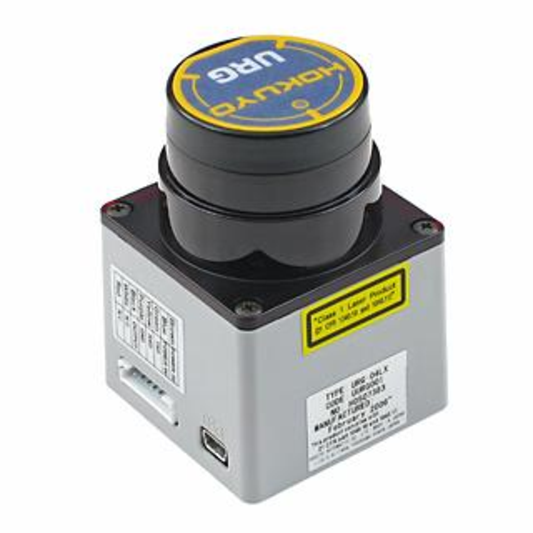
\includegraphics[scale=0.2295]{images/Hokuyo}};
		\node at (6,0) [draw=white,ultra thick,inner sep=0pt] {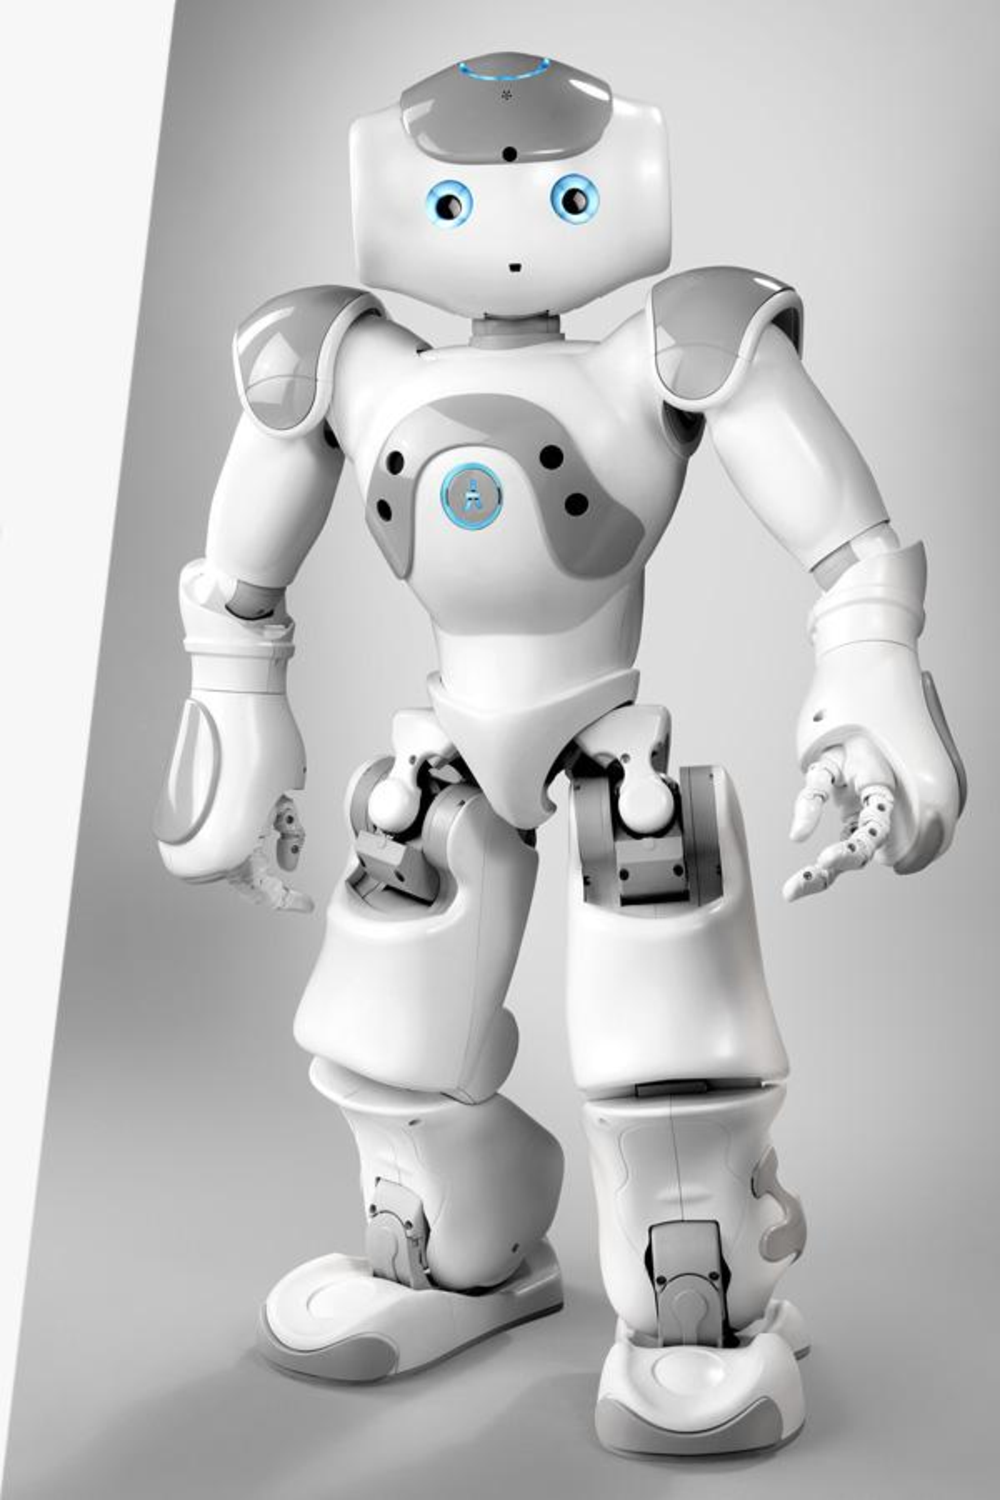
\includegraphics[scale=0.0815]{images/Nao}};
		\node at (8.3,0) [draw=white,ultra thick,inner sep=0pt] {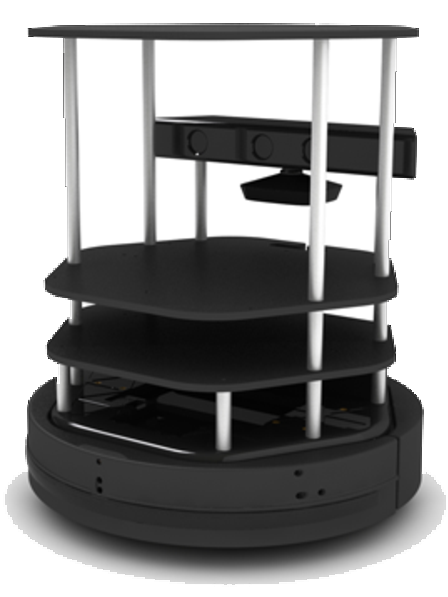
\includegraphics[scale=0.205]{images/Turtlebot}};
	\end{tikzpicture}
	
	\vspace{-1.8cm}
	
	\begin{tabbing}
		\hspace*{7.2cm}
		\Large
		\textbf{+}
	\end{tabbing}
	
	\vspace{0.6cm}
	
	\begin{tikzpicture}
		\node at (0,0) [draw=white,ultra thick,inner sep=0pt] {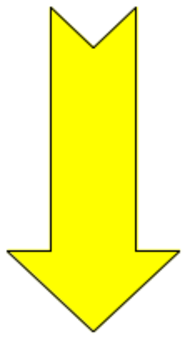
\includegraphics[scale=0.25]{images/ArrowDown}};
	\end{tikzpicture}
	
	\begin{block}{Ultimate Goal}
		Creating a distributed \textbf{lifelong} system able to continuously track the objects in an environment
		using multiple sensors and that is \textbf{able to learn} the behaviors of the tracked objects
	\end{block}
\end{frame}

\begin{frame}
	\frametitle{Related work}
	
	\vspace{0.5cm}
	
	Works that have significantly contributed to the improvement of one or more aspects of multiple target tracking.
	
	\begin{itemize}
		\item a synchronous algorithm based on the exchange of \emph{Gaussian Mixture Models} parameters that are
			  evaluated using a distributed \emph{Expectation-Maximization} method \cite{Gu07}
		\item a distributed approach that clusterizes the particle cloud in order to detect the targets'
			  poses \cite{Wu08}
		\item an asynchronous approach where the posterior probability is evaluated using a gossiping protocol for
			  data dissemination \cite{Oreshkin10}
	\end{itemize}
	
	\vspace{0.5cm}
	
	\tiny 1. \emph{Gu et al., ``Distributed particle filter for target tracking'' in ICRA 2007} \\
	\vspace{0.1cm}
	\tiny 2. \emph{Oreshkin et al., ``Asynchronous distributed particle filter via decentralized evaluation of Gaussian products''} \\
	\vspace{0.05cm}
	\tiny \emph{in Information Fusion (FUSION), 2010}\\
	\vspace{0.1cm}
	\tiny 4. \emph{Wu et al., ``Boosted Interactively Distributed Particle Filter for automatic multi-object tracking'' in 15th IEEE} \\
	\vspace{-0.18cm}
	\tiny \emph{International Conference on Image Processing, 2008}
\end{frame}
